\chapter{GIS.lab}
\label{2-teorie}

\begin{figure}[H] \centering
    
\includegraphics[width=80pt]{./pictures/gislab-logo.png}
    \caption[GIS.lab logo]{GIS.lab logo (zdroj:
	\href{https://github.com/gislab-npo/gislab-doc/blob/master/img/logo.svg}{GIS.lab repozitář})}
	\label{fig:gislab-logo}
\end{figure}

\section{Co je to GIS.lab?}
% https://gislab.readthedocs.io/en/latest/general/about.html
% http://geo.fsv.cvut.cz/~landa/publications/2016/telc-2016/prezentace/landa-telc-2016.pdf
% http://gislab-npo.github.io/gislab/index.html

GIS.lab je nástroj pro jednoduché a rychlé nasazení (deployment)
funkční, centrálně spravované \zk{GIS} infrastruktury v jednotném
prostředí lokální sítě (\zk{LAN}), v data centru nebo v cloudové
službě. Jedná se o technologii, která poskytuje komplexní soubor
otevřených GISových softwarových nástrojů integrovaných do jednoho
celistvého systému, jenž vyžaduje minimální náklady na
pořízení a údržbu. 

\begin{figure}[H] \centering
    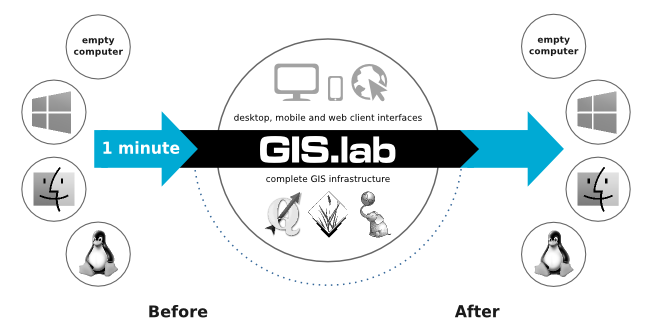
\includegraphics[width=400pt]{./pictures/gislab-schema.png}
    \caption[Schéma jednoduchosti nasazení GIS.lab]{Schéma jednoduchosti nasazení GIS.lab (zdroj:
	\href{https://github.com/gislab-npo/gislab-doc/blob/master/img/general/gislab-schema.png}{GIS.lab repozitář})}
	\label{fig:gislab-schema}
\end{figure}

Svět softwaru založeného na myšlence open-source sestává z velkého
množství různorodých osobností a skupin, z nichž každá svůj projekt
uchopuje po svém. Propojit tyto různorodé nástroje mezi sebou do
funkčního celku je náročný úkol a právě ten se pokouší řešit platforma
GIS.lab.

K největším výhodám této platformy patří maximálně automatizovaná
instalace či rychlé nasazení pomocí GIS.lab Unit (viz
\ref{gislab-unit}), jejichž výsledkem je plně funkční a vysoce výkonný
nástroj, bez nutnosti dalšího složitého nastavení. Přizpůsobení
specifickým potřebám zákazníka je však také možné.\footnote{Úpravy pro
  skupinu GISMentors:
  \href{https://github.com/GISMentors/gislab-customization}{https://github.com/GISMentors/gislab-customization}}
Všichni klienti GIS.labu Desktop, uživatelské účty i zálohy jsou
centrálně spravované.

Z hlediska \zk{GIS} infrastruktury a její komplexnosti jsou
nejzásadnější ukládání prostorově i neprostorově orientovaných dat (v
souborovém systému nebo v PostGIS databázi) a jejich sdílení, tvorba a
analýza vektorových, rastrových i tabulkových dat nebo rychlé
vytváření kartografických výstupů.

Desktopový klient (tlustý klient) GIS.lab Desktop může být spuštěn v
režimu fyzickém či virtuálním. Virtuální režim lze využít na
kterémkoliv operačním systému (\zk{OS}) s tím, že původní \zk{OS} i
GIS.lab jsou přístupné. Fyzický režim umožňuje lepší výkon, který je
vykoupen dočasnou nedostupností původního \zk{OS}.

\begin{figure}[H] \centering
    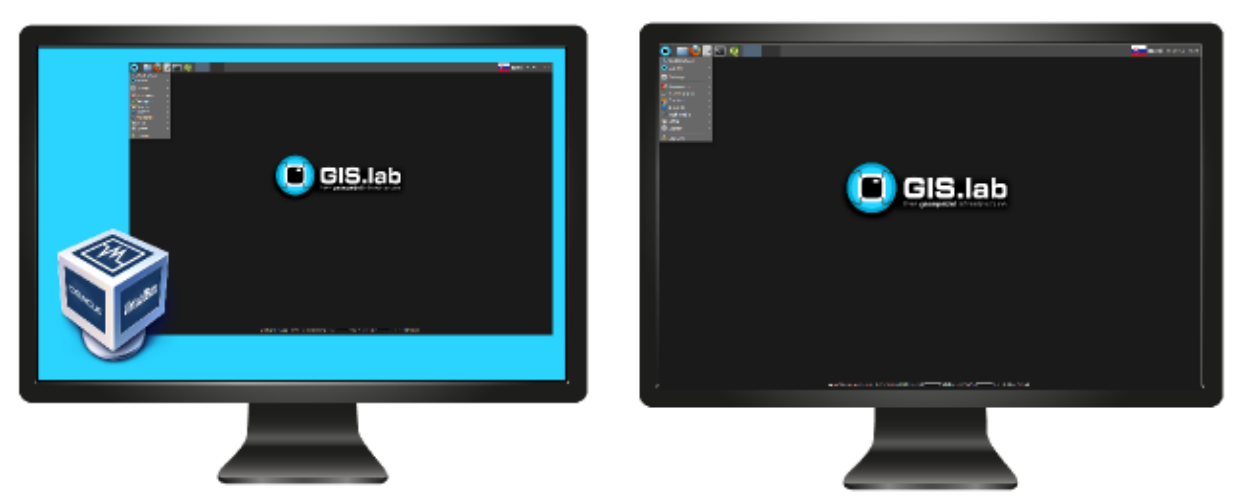
\includegraphics[width=450pt]{./pictures/physical-or-virtual-mode.png}
    \caption[Virtuální a fyzický režim GIS.lab Desktop]{Virtuální a fyzický režim GIS.lab Desktop (zdroj:
	\href{https://github.com/gislab-npo/gislab-doc/blob/master/img/installation/physical-or-virtual-mode.png}{GIS.lab repozitář})}
	\label{fig:gislab-rezim}
\end{figure}

Tlustý klient poskytuje desktopové prostředí bez zádrhelů, které by se
mohly vyskytovat u odlehčené webové verze. Jeho využití však není primárně
zamýšleno v tradičním pojetí desktopu jako jediného klienta, ale spíše
jako jakési specializované klientské rozhraní poskytující nástroje ze
světa desktopu.

Konfiguraci a nasazení GIS.labu řídí platforma Ansible (viz
\ref{docker}). Deployment ve virtuálním režimu umožňuje
Vagrant\footnote{open-source nástroj pro vytváření a údržbu
  přesnosného vývojového prostředí pomocí virtualizace} a
VirtualBox\footnote{Oracle VM VirtualBox, multiplatformní
  virtualizační nástroj}.

GIS.lab se po nasazení sestává z jednoho stroje, který zastává roli
hlavního uzlu (server, master), a k němu připojeného množství dalších počítačů
(klientů, nodes). Výsledkem je lokální počítačová síť, v podstatě jakýsi cluster.
Pro hlavní uzel je vyžadován stroj, který běží na operačním systému
Ubuntu či se na něj dá doinstalovat, požadavky na klientské počítače nejsou téměř žádné - nemusí
obsahovat operační systém ani pevný disk. Je však potřeba, aby všechny
počítače v síti byly připojené pomocí gigabitového síťového kabelu a
síťového přepínače (switch). Výpočetní kapacitu je možné sdílet přes všechny stroje.

\begin{figure}[H] \centering
    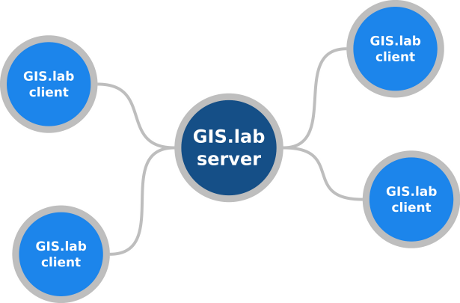
\includegraphics[width=280pt]{./pictures/gislab-architecture.png}
    \caption[GIS.lab architektura]{GIS.lab architektura (zdroj:
	\href{https://github.com/gislab-npo/gislab-doc/blob/master/img/general/gislab-architecture.png}{GIS.lab repozitář})}
	\label{fig:gislab-architecture}
\end{figure}

GIS.lab Server běží na operačním systému Ubuntu Linux LTS s odlehčeným
desktopovým prostředím XFCE.  K ověření a správě uživatelů využívá
protokol LDAP, přesněji jeho nadstavbu OpenLDAP (viz \ref{openldap}).

%https://gislab.readthedocs.io/en/latest/client-layout/index.html#gis-applications
Vedle základního softwarového vybavení standardního \zk{OS} jsou
dostupné dva hlavní GISové programy QGIS a GRASS GIS. QGIS je vhodný
pro tvorbu projektů, přípravu a analýzu dat. Umožňuje i jejich
následnou publikaci nejen v podobě \zk{WMS}/\zk{WFS} služeb, ale i
jako webových aplikací pomocí předinstalovaného zásuvného modulu
Gisquick. GRASS GIS lze využít pro komplexní datové analýzy.

Data jsou uložena v souborovém systému či geodatabázi
PostGIS. Dostupná je i nadstavba SpatiaLite pro databázi SQLite
umožňující ukládání geoprostorových dat.

GIS.lab obsahuje velké množství knihoven a balíčků Python, z nichž zde
jsou zmíněni jen vybraní zástupci. GDAL je knihovna určená pro zápis a
čtení vektorových a rastrových geodat. Proj.4 slouží k transformaci
geoprostorových souřadnic z jednoho souřadnicového systému do
dalšího. Pro práci se satelitními daty družic MODIS a Sentinel slouží
PyModis a Sentinelsat.
% přidat JOSM?

Přizpůsobení základní instalace specifickým požadavkům může být
provedeno buď standardními linuxovými příkazy, nebo upravením Ansible
Playbooks, které se vyznačují pro člověka snadno čitelným
jazykem. Chování systému během vytváření a odstraňování uživatelských
účtů je definováno v pěti speciálních skriptech.
\begin{itemize}
\item \texttt{before-add} - spuštěn před vytvořením účtu
\item \texttt{after-add} - spuštěn po vytvoření účtu
\item \texttt{before-delete} - spuštěn před odstraněním účtu
\item \texttt{after-delete} - spuštěn po odstranění účtu
\item \texttt{files} - obsah tohoto adresáře je zkopírován do domovského adresáře uživatele předtím než je spuštěn skript \texttt{after-add}
\end{itemize}
Tyto skripty je také možné upravovat konkrétním potřebám. Příkladem
může být nakládání s databází. Ve skriptu \texttt{after-add}
definujeme, zda uživateli bude vytvořena nová databáze nebo jen
přidáno schéma do již existující společné. Ve skriptu
\texttt{before-delete} zvolíme, jestli před odstraněním účtu dojde k
vyprodukování tzv. dumpu, který bude uživateli zaslán na jeho
adresu. A nakonec při spuštění \texttt{after-delete} bude tato
databáze/schéma odstraněno.

\subsubsection{GIS.lab Unit}
\label{gislab-unit}
%http://gislab-npo.github.io/gislab/pages/gislab-unit
Zařízení s názvem GIS.lab Unit je přenosné hardwarové řešení
obsahující systém GIS.lab připravený k okamžitému zapojení a nasazení
ve zvolené síti. Jedná se o krabičku s rozměry přibližně 11 x 11 x 4
cm, procesorem Intel Haswell, SSD diskem a 16 GB RAM. Maximální
testované množství klientských počítačů je 20, v rámci výuky na
Fakultě stavební ČVUT.

\begin{figure}[H] \centering
    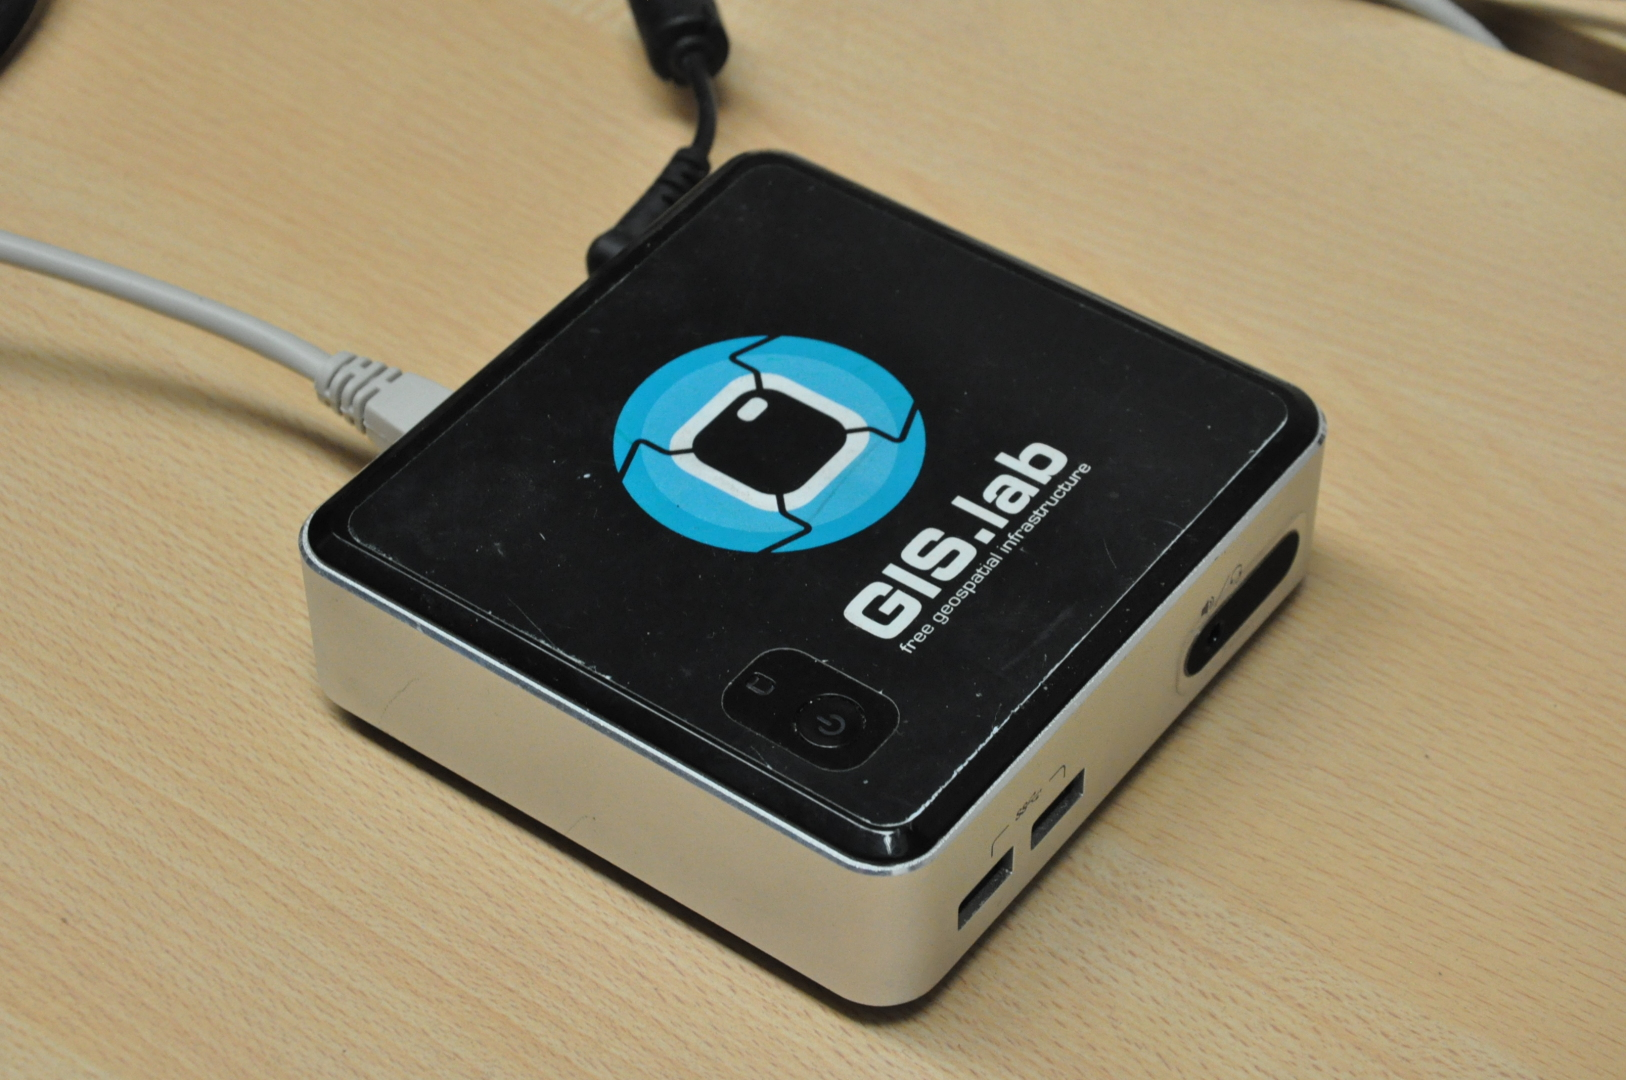
\includegraphics[width=350pt]{./pictures/gislab-unit.jpg}
    \caption[GIS.lab Unit]{GIS.lab Unit (zdroj:
	\href{http://gismentors.cz/wp-content/uploads/2018/12/DSC_0043.jpg}{GISMentors})}
    \label{fig:gislab-unit}
\end{figure}

S pomocí integrované platformy Gisquick (viz \ref{gisquick}) podporuje
GIS.lab kromě desktopového klienta i webovou publikační platformu.

\section{Gisquick}
\label{gisquick}
% http://gisquick.org - využila jsem 
% https://gisquick.readthedocs.io/en/latest/user-manual/project-publishing.html - nevyužila jsem 

\begin{figure}[H] \centering
    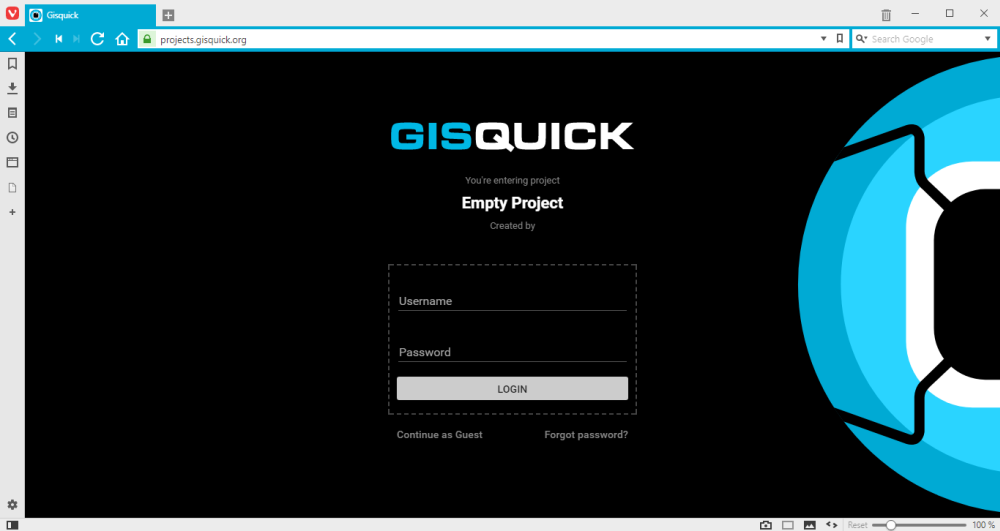
\includegraphics[width=400pt]{./pictures/gisquick-welcome-screen.png}
    \caption[Gisquick - přihlašovací stránka]{Gisquick - přihlašovací stránka (zdroj:
	\href{}{Tereza Kulovaná})}
    \label{fig:gisquick-welcome}
\end{figure}

Gisquick je open-source platforma umožňující publikaci geoprostorových
dat. Byla vytvořena s cílem snadného sdílení projektů vytvořených v
desktopové aplikaci QGIS na webu. Gisquick sestává ze zásuvného modulu
QGIS, QGIS serveru, serverové aplikace založené na frameworku Django a 
webového klienta. Obsahuje základní sadu nástrojů
potřebných pro webovou mapovou aplikaci s plně responzivním uživatelským
rozhraním (\zk{GUI}).

Gisquick byl vyvíjen jako součást GIS.labu, ale v roce 2015 se oddělil
jako samostatný projekt. Dle původní představy autorů měl mít Gisquick
podobu tenkého klienta GIS.labu, tedy jakési odlehčené verze. Měl 
nabízet nástroje pro interakci s daty - editaci, provádění výpočtů a analýz.
Aktuálně však umožňuje pouze jejich zobrazování. 

Dnes je možné ho využívat samostatně, zároveň však zůstává integrován 
v každé instalaci GIS.labu a rozšiřuje jeho funkcionalitu. Je distribuován 
pod otevřenou licencí GNU \zk{GPL} v2.0.

\section{Aktuální využití}
\label{gislab-vyuziti}

V současné době se GIS.lab využívá především při výuce na Fakultě
stavební ČVUT v rámci hodin zaměřených na \zk{GIS} a dálkový průzkum
Země (\zk{DPZ}) a na Přírodovědecké fakultě Univerzity Karlovy. Také
na něm probíhají veřejná školení skupiny GISMentors.

\begin{figure}[H] \centering
    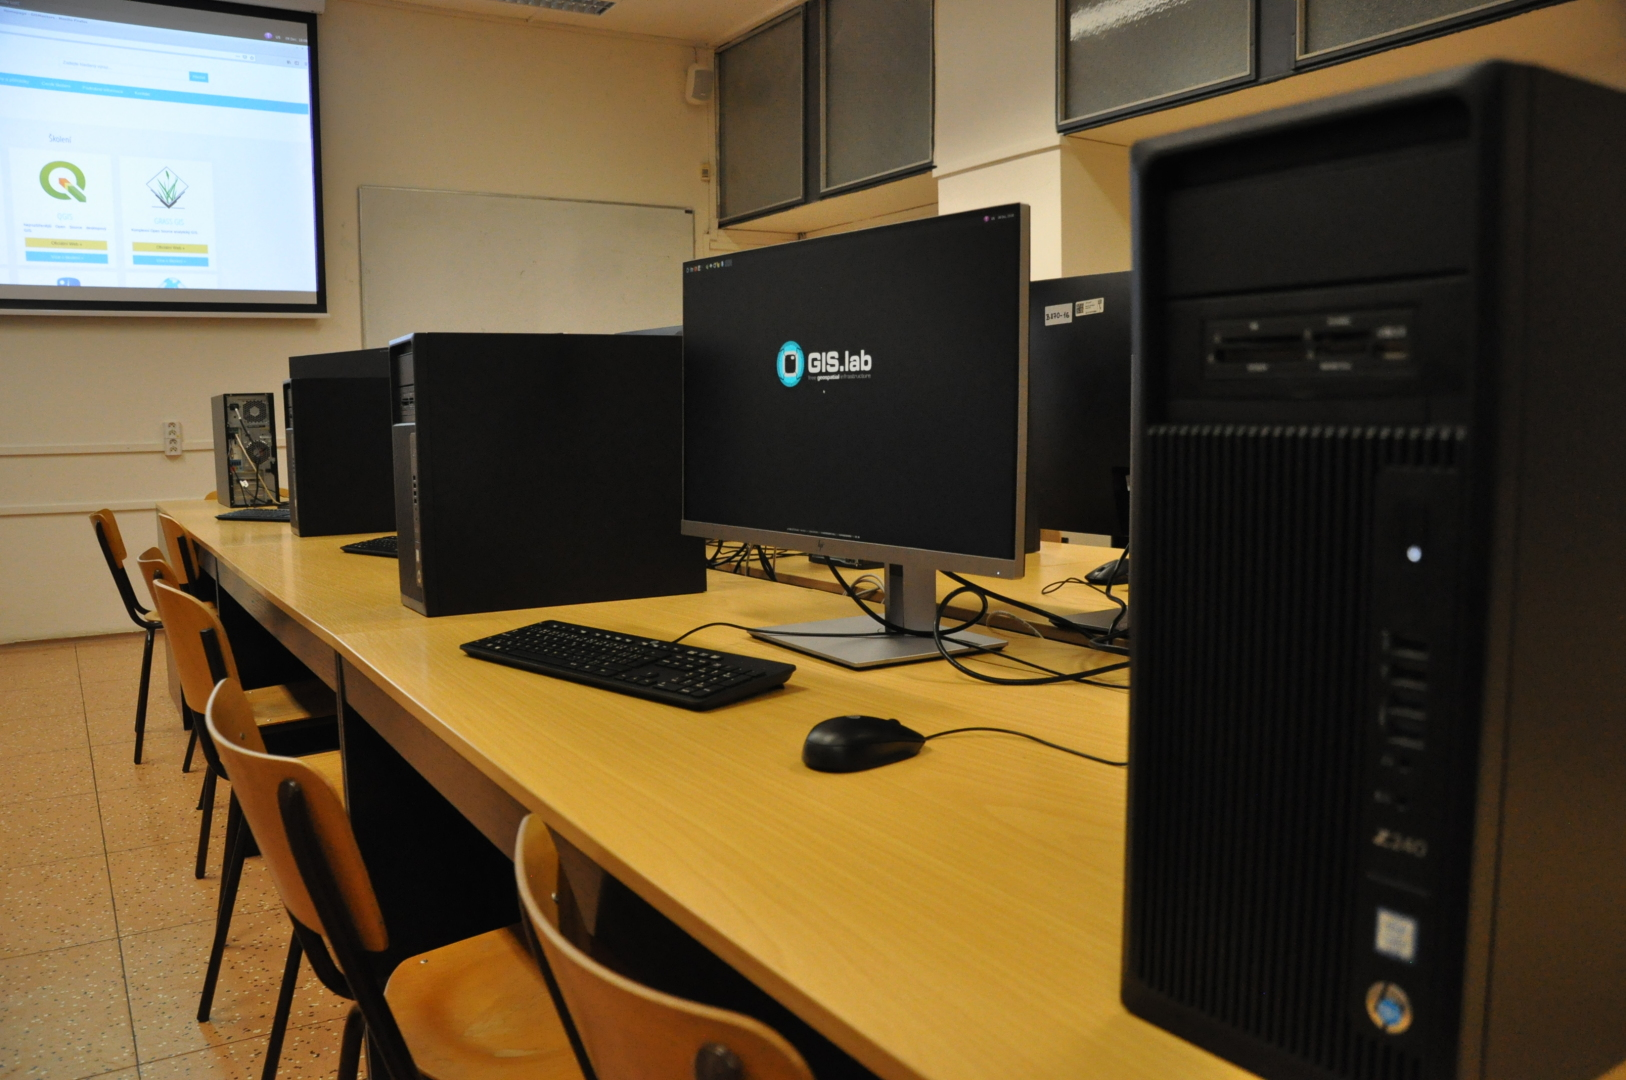
\includegraphics[width=350pt]{./pictures/classroom.jpg}
    \caption[Počítačová učebna Fakulty stavební ČVUT]{Počítačová učebna Fakulty stavební ČVUT (zdroj:
	\href{http://gismentors.cz/wp-content/uploads/2018/12/DSC_0051.jpg}{GISMentors})}
    \label{fig:gisquick-welcome}
\end{figure}

Vyučování na stavební fakultě probíhá ve fyzickém režimu GIS.lab Desktop s nasazením
pomocí GIS.lab Unit. Každý student má vytvořen vlastní uživatelský
účet a dedikované schéma v databázi. Studenti jsou seznámeni s
připojením k databázi pomocí PgAdmin, většinou je však využíváno
připojení přes QGIS. QGIS je také upřednostňovaným softwarem při
zpracování prostorových i neprostorových dat, výhodou je i možnost
využívat zásuvný modul Gisquick pro publikaci dat v podobě webových
aplikací. Studenti jsou krátce seznámeni s programem GRASS GIS,
strukturou GRASS projektů a práce s nimi. GRASS GIS je více využíván v
rámci předmětů orientovaných na \zk{DPZ}, jelikož obsahuje dobře
implementované nástroje pro zpracování obrazových dat. K nástrojům
GRASS GIS mohou uživatelé přistupovat i přes QGIS \zk{UI} díky
předinstalovanému zásuvnému modulu QGIS GRASS.

%TK: tohle možná přesunout nahoru k popisu? (někam před gislab Unit)
Komunikace probíhá přes zabudovanou IRC službu, kterou lze využít mimo
jiné pro okamžité a jednoduché sdílení nezbytných příkazů či
potřebných webových adres. Pro sdílení souborů jsou určené dvě složky,
k nimž mají přístup všichni připojení uživatelé. Pro standardní výměnu
mezi klientskými počítači je příhodnější složka \textit{Barrel} s
právy čtení i zápisu pro všechny. Data trvalejšího charakteru je
vhodné umístit do adresáře \textit{Repository}, odkud je možné data
stahovat, ale upravovat je mohou pouze správci.

\section{Plány na rozšíření}
\label{vision}

Autoři GIS.labu by rádi v budoucnu rozšířili uživatelskou základnu,
proto mají za cíl práci správcům i uživatelům zpříjemnit a nabídnout
co nejširší portfolio různých balíčků (tzv. services). 

\begin{figure}[H] \centering
    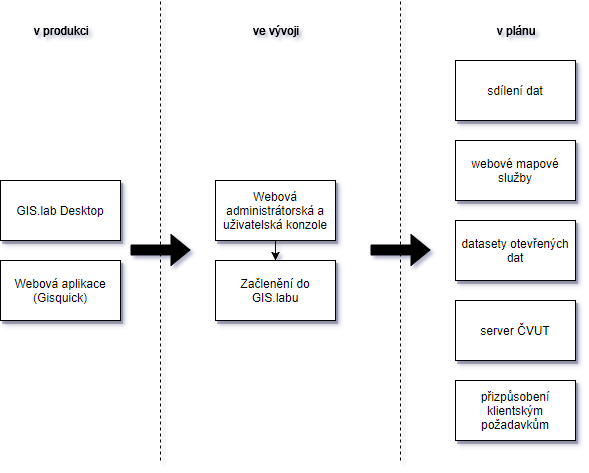
\includegraphics[width=350pt]{./pictures/gislab_road_map_02.png}
    \caption[Vývoj GIS.labu]{Vývoj GIS.labu (zdroj:
	\href{}{Tereza Kulovaná})}
    \label{fig:gislab-roadmap}
\end{figure}

\subsubsection{Webová administrátorská a uživatelská konzole}

Nejblíže zařazení na seznam služeb je webové rozhraní pro správu
uživatelů, které je zpracováváno v rámci této diplomové
práce. 

Aktuálně používaný systém správy uživatelů funguje na bázi příkazové
řádky a je popsán v kapitole \ref{cmd-line}. Tento systém není pro
všechny úplně intuitivní, zároveň neumožňuje přístup ze strany
uživatelů. Proto je cílem vytvořit webové grafické uživatelské
rozhraní (\zk{GUI}), které bude mít dvě části - administrátorskou a
uživatelskou.

Uživatelská konzole bude umožňovat registraci, přístup k osobním
údajům a jejich editaci a v neposlední řadě žádosti o zpřístupnění
jednotlivých balíčků služeb. Balíčky by v první fázi měly sestávat z
pěti složek: datasetů otevřených dat; přístupu k datům (souborový
systém, DB); publikace dat pomocí webových mapových služeb; webové
aplikace; desktopového klienta. Přístup k prvním třem komponentám by
měl být možný i mimo desktopového klienta, což je další důvod pro
vytvoření webového rozhraní, ke kterému lze přistupovat z jakéhokoliv
počítače. Přes konzoli bude probíhat i sdílení dat s dalšími uživateli
či žádost o navýšení kapacity databáze. Kromě úpravy uživatelských
údajů budou všechny změny vyžadovat potvrzení správce.

Administrátorská konzole bude mít v podstatě stejnou funkcionalitu
jako uživatelská s tím rozdílem, že administrátor bude moci spravovat
všechny uživatele.

\begin{figure}[H] \centering
    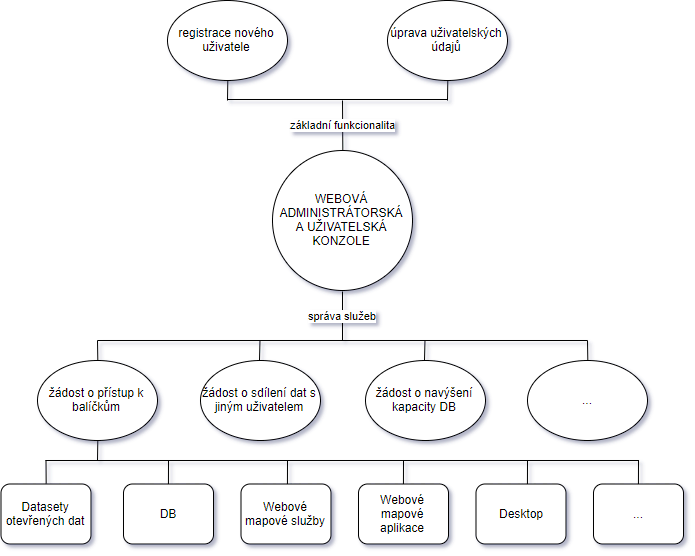
\includegraphics[width=400pt]{./pictures/console_services_02.png}
    \caption[Budoucí podoba webové konzole]{Budoucí podoba webové konzole (zdroj:
	\href{}{Tereza Kulovaná})}
    \label{fig:konzole-sluzby}
\end{figure}

\subsubsection{Sdílení dat}
V případě fyzického režimu GIS.lab Desktop jsou veškerá vytvořená data
dostupná pouze v rámci klienta, na němž GIS.lab běží, sdílet s dalšími
uživateli je lze pouze přes společné adresáře \textit{Repository} a
\textit{Barrel}. Data jsou tímto způsobem přístupná všem uživatelům v
rámci sítě bez rozdílu.

Pokud by se chtěl uživatel podělit o přístup k některé části své
databáze, bude k tomu moci v první fázi využít SQL příkazu GRANT,
později pak vyhledat jiného uživatele přes webovou administrátorskou
konzoli a přístup mu udělit přes ni.

Virtuální režim GIS.lab Desktop běží nad VirtualBoxem, který umožňuje 
připojení složek z hostitelského \zk{OS}. Pokud má uživatel zájem data 
přenést z fyzického klienta pryč nebo naopak nějaká
data nahrát, musí k tomu využít mezistupeň v podobě externího disku,
ať už reálného či virtuálního. Ideální by proto byla možnost
přistupovat vzdáleně nejen k databázi, ale například i k oddílu na
serveru obsahujícím data ve formátu Esri Shapefile (.shp) či OGC
GeoPackage (.gpkg). Tuto variantu bude umožňovat sdílení pomocí služby
NFS (Network File System). Tímto způsobem budou moci uživatelé
pracovat s daty i při běhu svého standardního \zk{OS}.

Desktopový klient již \zk{NFS} využívá pro připojení některých adresářů 
(Home, Barell, Repository) ze serveru. Cílem tedy je povolit sdílení 
disku i mimo desktop klienta.

\subsubsection{Webové mapové služby}
Pro publikaci dat je nyní aktuálně nutné být přihlášen na desktopovém
klientovi GIS.lab, zde vytvořit projekt a nakopírovat jej do adresáře
\textit{Publish}. Poté je přístupný jako webová služba dle standardu
OGC (Open Geospatial Consortium). Cílem je umožnit uživateli vytvořit
si projekt ve svém vlastním prostředí a následně ho jen nahrát na
server, který by dovolil jeho sdílení. Připojení k serveru za tímto
účelem bude umožňovat výše zmiňovaná služba \zk{NFS}.

Další variantu bude pro uživatele nabízet webová uživatelská konzole,
přes níž bude možné projekt na server nahrát a konzole zpátky
klientovi vygeneruje správnou cestu k webové mapové službě. Tento
přístup bude potřeba zvláště v případě, že uživatel bude mít přístup
pouze k balíčku webových mapových služeb.

\subsubsection{Datasety otevřených dat}

Část dat už je dnes v rámci státní správy České republiky poskytovaná ve
formě otevřených dat. Ne všichni uživatelé, kteří by je mohli ke své 
práci využít, však vědí, kde zmiňovaná
data najít, případně jak je dostat do formátu vhodného k dalším
analýzám. Právě pro ně bude vhodný další balíček.

Pokud si to správce zvolí, GIS.lab server bude obsahovat stažená
geoprostorová data, především z Českého úřadu zeměměřického a
katastrálního (ČÚZK) - územní jednotky, Registr územní identifikace,
adres a nemovitostí (RÚIAN), apod. Na datové sady budou po stažení
aplikovány testy datové integrity, případné nekonzistence budou
odstraněny a výsledek bude začleněn do PostGIS databáze. Přístup 
k těmto datasetům bude možný i nezávisle na jakémkoli dalším balíčku.

Konkrétní datové sady a tempo jejich aktualizací budou rozhodnuty až
při reálné implementaci.

\subsubsection{Server ČVUT}
Snaha o rozšíření základny uživatelů platformy GIS.lab cílí v
nejbližší době především na studenty a zaměstnance ČVUT a to i mimo Fakultu
stavební. V prvním kroku již byly získány prostředky, jež umožňují
spuštění GIS.labu přes server ČVUT. Pro jednotlivé fakulty či katedry,
které by se jej rozhodly využívat, bude připraveno několik základních
přizpůsobení, hlavně s ohledem na datasety z veřejného sektoru.

\subsubsection{Přizpůsobení klientským požadavkům}
Poslední v blízké době plánovanou změnou je umožnit zákazníkům
přizpůsobit platformu GIS.lab konkrétním požadavkům již při nasazení
pomocí Ansible Playbooks (viz \ref{docker}). Aktuálně jsou využívány
pro plně automatizovanou instalaci základní podoby GIS.labu a úpravy
pro jednotlivá školení skupiny GISMentors. Podobným způsobem jako pro
GISMentors se bude uzpůsobovat prostředí i pro další skupiny,
např. fakulty ČVUT.

Ukázky nejvyužívanějších nastavení budou dostupné v Github
repozitáři 
\href{https://github.com/gislab-npo/gislab/}{https://github.com/gislab-npo/gislab/}.

